To improve covariate balance between treated and control firms, and hence precision, I estimate a propensity score for flood exposure using pre-determined firm and location characteristics, following a specification similar to \cite{fatica2024floods}.

As long as unconfoundedness is assumed and common support is established, IPW estimators can be used to estimate ATE and ATT effects. While ATE weights ask what would happen if a randomly selected firm were flooded, ATT weights estimate how floods affected firms that were actually flooded. Given my interest in realized flood shocks, I focus on the ATT. I examine the distribution of the propensity score across treatment status. I then use the score to construct analytical weights. The ATT weights are of the form:

\noindent\text{weights given by}
\begin{align*} w_1^{att}(D) &= \frac{D}{\mathbb{E}[D]}, \\ w_0^{att}(D, p(X)) &= \frac{\frac{(1 - D)p(X)}{1 - p(X)}}{\mathbb{E}\left[ \frac{(1 - D)p(X)}{1 - p(X)} \right]}. \end{align*}

I begin with a pooled logit that relies only on time-invariant firm characteristics, whose result is presented in Table \ref{tab:pscore_logit}. Once the propensity score is known, I build the ATT weights as described above and proceed with standard inference procedures, re-estimate the outcome model on this re-weighted sample. The distribution of $p(x)$ in the adjusted and unadjusted sample is shown in Figure \ref{fig:pscore_distr}, while Figure \ref{fig:ps_cov_balance} illustrates the improvement in covariate balance achieved by the computed weights.

\vspace{1cm}

\begin{table}[!htbp] 
\centering 
\caption{\textbf{Table \ref{tab:pscore_logit}:} \textsc{Propensity-score logit for extreme floods (2010–2019)}} 
\label{tab:pscore_logit}

 \resizebox{12cm}{!}{
\begin{tabular}{@{\extracolsep{6pt}}p{8cm} c} 
\\[-1.8ex]\hline 
\hline \\[-1.8ex] 
& \textit{Dependent variable:}\\ 
\cline{2-2} 
\\[-1.8ex] & Extreme-flood dummy\\ 
\hline \\[-1.8ex] 
Flood–risk-group decile            & 0.160$^{***}$ \\ 
                                   & (0.029)        \\[0.15em]

Share of establishments under EAIP & 0.219          \\ 
                                   & (0.280)        \\[0.15em]

Income category of commune         & 0.0334         \\ 
                                   & (0.088)        \\[0.15em]

Urban dummy                        & 0.456$^{***}$  \\ 
                                   & (0.073)        \\[0.15em]

Coastal dummy (littoral sea)       & 0.908$^{***}$  \\ 
                                   & (0.127)        \\[0.15em]

Floods 1982–1999 (count)           & $-$0.118$^{***}$ \\ 
                                   & (0.044)        \\[0.15em]

Constant                           & $-$3.476$^{***}$ \\ 
                                   & (0.206)        \\[0.35em]
\hline \\[-1.8ex] 
Observations                       & 6,676,631       \\ 
Wald $\chi^2$(6)                   & 178.33          \\ 
Pseudo R$^2$                       & 0.0293          \\ 
Log pseudolikelihood               & $-$1,564,659.3  \\ 
\hline 
\hline \\[-1.8ex] 
\multicolumn{2}{p{13cm}}{\textit{Note:} $^{*}p<$0.1; $^{**}p<$0.05; $^{***}p<$0.01. Robust standard errors clustered at the commune level. Coastal dummy includes only sea-type areas (89\% of cases). Interestingly, the coefficient for floods occurring in 1982–1999 is negative, possibly indicating that adaptation to flooding has taken place in communes more heavily exposed in the past, now resulting in fewer CatNat declarations.} \\ 
\end{tabular}}
\end{table}

% , the next steps are: 1) convert the obtained propensity scores to IPW (ATE) or ATT weights, then compute MSD in the IPW-weighted data so that treated and control groups share the same covariate distribution, and ; 2) apply doubly-robust IPW-RA; 3) nearest-neighbor matching, pairing each flooded commune with the dry commune that has the closest propensity score and computing the mean outcome gap within those matched pairs; 4) drop units whose predicted score is near 0 or 1, keeping only the range where both treated and control communes exist, then run the analysis on that trimmed sample.

% Since I cannot estimate ATE (there is selection into treatment), I estimate ATT effects. The weights are built as $\frac{e_i}{1-e_i}$ for controls. Balance is shown after matching.



% \noindent To capture common calendar-year shocks and unobserved heterogeneity across firms, one could also estimate a more nuanced model such as:

% \begin{equation}
% \Pr!\bigl(D_{it}=1 ,\big|, X_i, T_t, u_i\bigr)=
% \Phi!\Bigl(\alpha X_i+\delta T_t+u_i\Bigr)
% \end{equation}

% This would allow estimation of a more accurate propensity score.


\begin{figure}[htbp]
\centering
\caption{\textbf{Figure \ref{fig:ps_cov_balance}:} Covariate balance before and after matching}
\label{fig:ps_cov_balance}
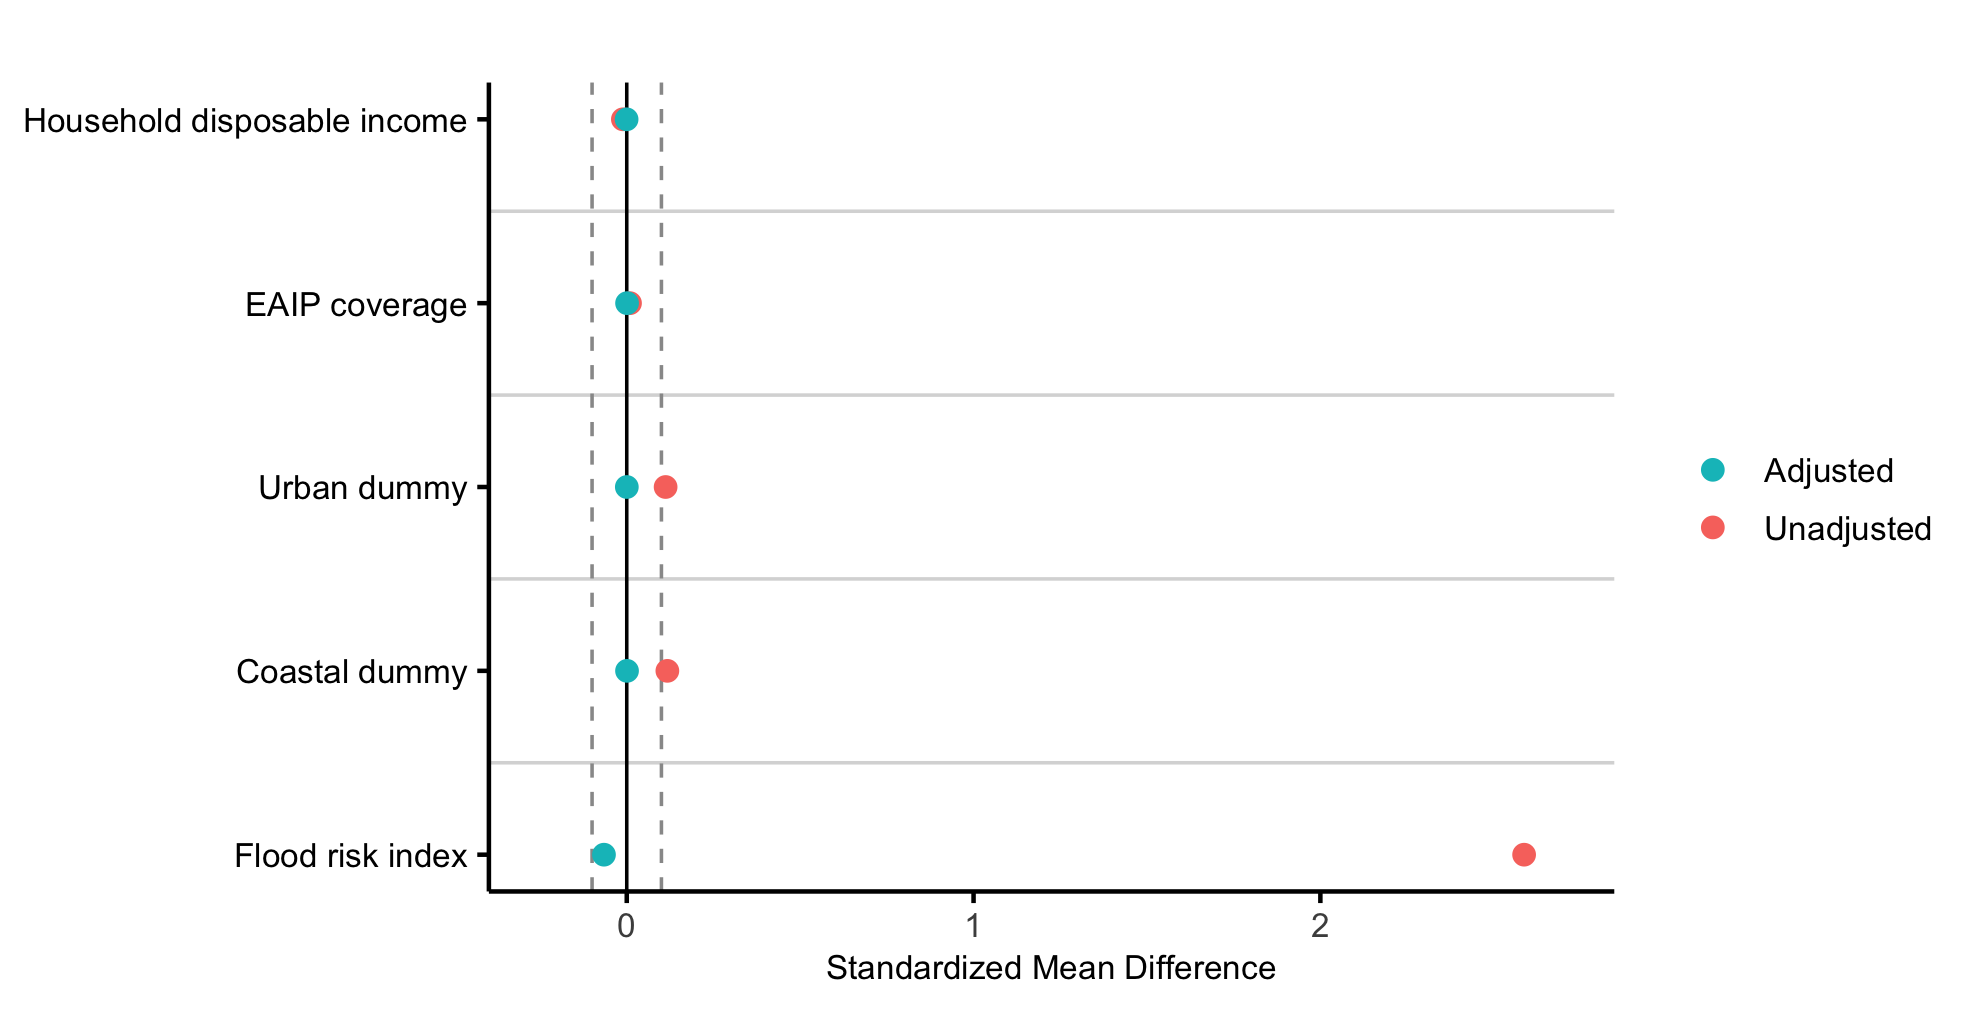
\includegraphics[width=0.86\textwidth]{figures/PScore/covariate_balance.png}
\caption*{\raggedright\textit{Note}: Flood risk index is an outlier with 2.59 SMD in the unadjusted sample.}
\end{figure}

\vspace{0.2cm}

\begin{figure}[htbp]
\centering
\caption{\textbf{Figure \ref{fig:pscore_distr}}: Propensity score distribution}
\label{fig:pscore_distr}
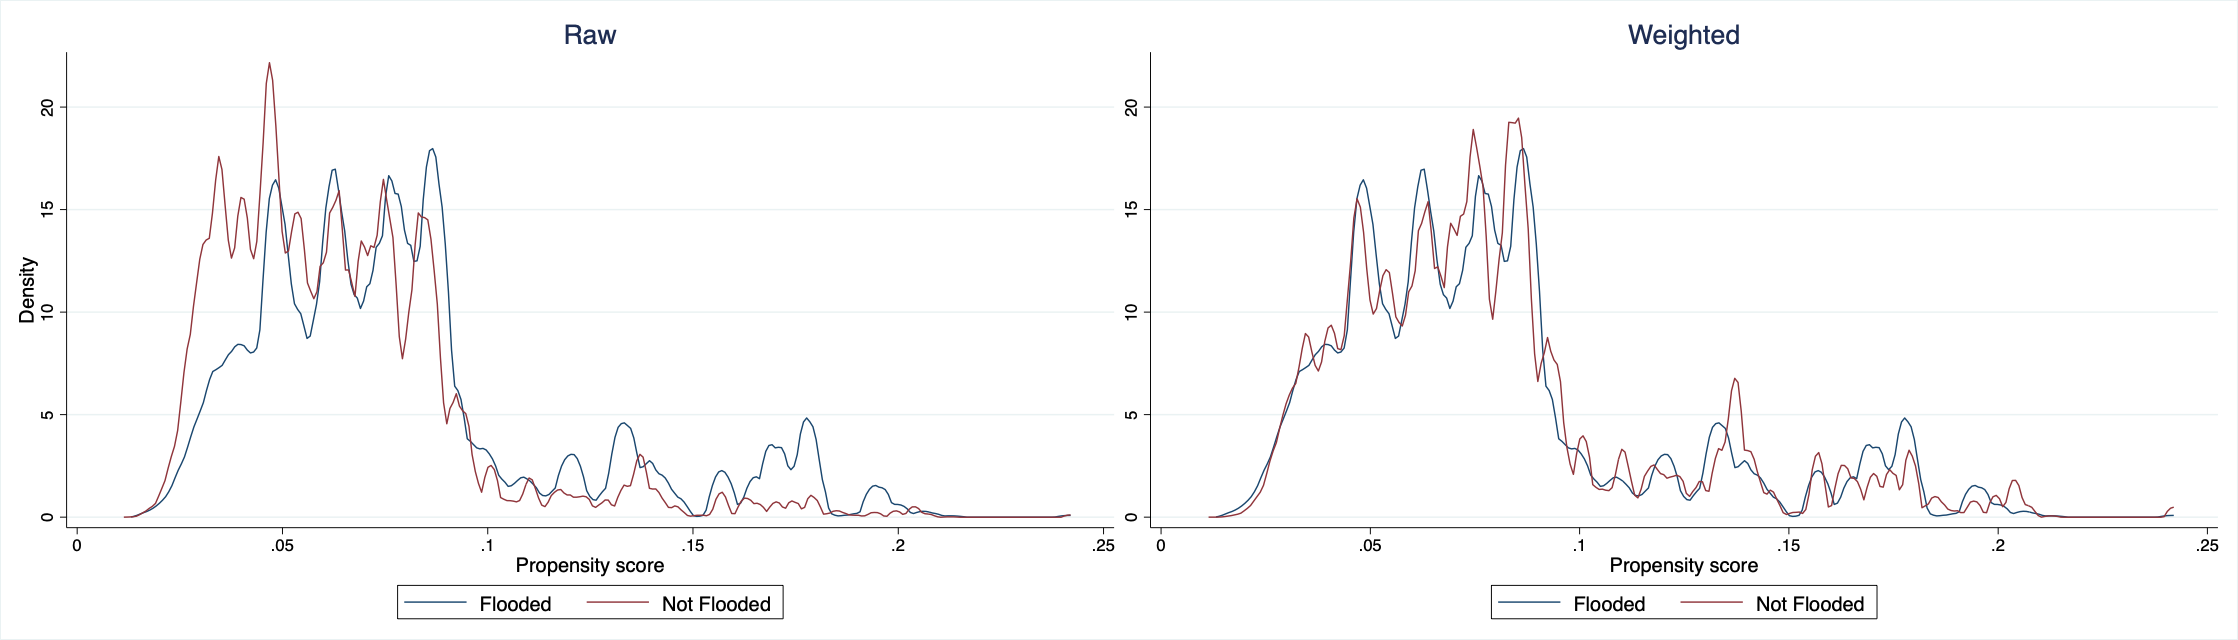
\includegraphics[width=1\textwidth]{figures/PScore/pscore_distrib.png}
\caption*{\raggedright\textit{Note}: The figure displays the distributions of the propensity scores before and after weighting, restricted to the region of common support. 2.12\% of the sample (N=144,299) is excluded because it is not in common support.}
\end{figure}